\subsection{Hierarchical clustering}
\draft{da scrivere}

\draft{hierarchical clustering}
Hierarchical clustering is a general family of clustering algorithms that build nested clusters by merging or splitting them successively. This hierarchy of clusters is represented as a tree (or dendrogram). The root of the tree is the unique cluster that gathers all the samples, the leaves being the clusters with only one sample. See the Wikipedia page for more details.

The AgglomerativeClustering object performs a hierarchical clustering using a bottom up approach: each observation starts in its own cluster, and clusters are successively merged together. The linkage criteria determines the metric used for the merge strategy:

Ward minimizes the sum of squared differences within all clusters. It is a variance-minimizing approach and in this sense is similar to the k-means objective function but tackled with an agglomerative hierarchical approach.
Maximum or complete linkage minimizes the maximum distance between observations of pairs of clusters.
Average linkage minimizes the average of the distances between all observations of pairs of clusters.
Single linkage minimizes the distance between the closest observations of pairs of clusters.
AgglomerativeClustering can also scale to large number of samples when it is used jointly with a connectivity matrix, but is computationally expensive when no connectivity constraints are added between samples: it considers at each step all the possible merges.
\begin{lstlisting}[style=mypython]
from sklearn.cluster import AgglomerativeClustering
AgglomerativeClustering(
    affinity='euclidean',
    compute_full_tree='auto',
    linkage='ward',
    n_clusters=x,
    )
\end{lstlisting}

\subsection{LDA}\label{sec:lda}
\draft{commenti vari}
As in ~\cite{Zhou2016}
\begin{equation}\label{eq:lda}
P(w, z,\beta, \theta| \alpha, \eta)=\prod_n^{N_d} P(w|z,\beta)P(z|\theta)\prod_k^KP(\beta|\eta)\prod_d^N P(\theta | \alpha)
\end{equation}

\begin{figure}
	\centering
	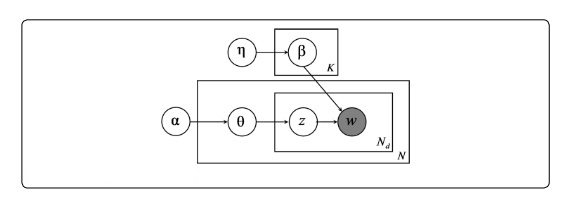
\includegraphics[width=0.5\linewidth]{pictures/topic/LDA.jpeg}
	\label{fig:LDA}
	\caption{LAD scheme}
\end{figure}
where
\begin{itemize}
	\item $N$ number of documents
	\item $K$ number of topics
	\item $w$ words
	\item $N_d$ number of words in document d
	\item $\eta$ and $\alpha$ are parameters of the model
\end{itemize}
in~\ref{eq:lda} $P(\theta | \alpha)$ and $P(\beta|\eta)$ are Dirichlet distributions the outputs are the topic distribution in documents $P(z|d)$ and the word distribution in topics $P(w|z)$